% --------------------------------------------
%		CAPITOLO 5
%---------------------------------------------

\chapter{TJ-Monopix 2 characterization ??}
%\addcontentsline{toc}{chapter}{Caratterizzazione di TJ-Monopix 2}

\section{Matrix and flavors}

\subsection{Mask (operation) and noisy pixels}

\subsection{Analog and digital readout}

\subsubsection{BCID reset}
\begin{comment}
REFERENZE
\end{comment}

\subsubsection{Main registers (and conversion?)}

\subsection{Comparison of trends from data with simulation}
%\addcontentsline{toc}{subsection}{Confronto degli andamenti con le simulazioni}


\section{Characterization by injection}
%\addcontentsline{toc}{section}{Caratterizzazione tramite l'iniezione}

In the prototype under test (study), W14R12 chip, some problems (raised up) arose right from the beginning, linked (concerned) pixels of the matrix both for the analog and digital part.
Despite its predecessor Tj-Monopix 1, Tj-Monopix 2 is equipped with a circuit which allows the \textit{threshold tuning}.In other words it can adjust, even if only few DAC, every pixel threshold, in order to have a global threshold on the matrix as uniform as possible, or in any case a dispersion as small as possible.

Preliminarly it's necessary to study the threshold distribution on the whole matrix. We have separately analyzed the four flavors, to be able to study their main difference in working (performance) and features.

The ultimate purpose of this measurement is to describe (depict, mark out) the behaviour of each pixel, injecting a charge equivalent to the typical energy released from electrons emitted in radioactive decays (decays of radioactive materials) and in particular those produced by the electronic capture of \ch{^{55}Fe} (presente in laboratorio). As explained in the previous section (reference), the \ch{^{55}Fe} has an emission spectrum (lines) with lines quite peaked (sharp) and this allows to compare data more easily. The first line is at 5.9 KeV which corresponds on average to about 1616 $e^{-}$ released (through the pixel??).
For this reason during the injection measurement, it's mandatory to know the conversion between DAC and $e^{-}$ (reference) and to inject charges in order to study pixel behaviour  the right region, which are more interesting from a physical point of view.

\begin{figure}[h!]
\centering
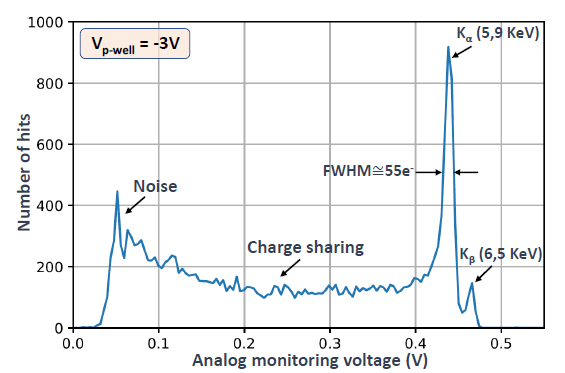
\includegraphics[scale=0.8]{spectrum_fe}
\caption{\ch{^{55}Fe} (radiactive source) emission spectrum using the analog output of a PMOS reset front-end of TJ-Monopix 1. (referenceeeeee)}
\label{fig:fespectrum}
\end{figure}

%------------------------------------------------------------
\subsection{Injection circuit issues}

In carrying out the measurements mentioned above, we noticed (NO) some issues with the injection circuit which limits its working range: (as a matter of fact) the height of the injection pulse is expected to grow (increase) linearly up to a value of (about) $\approx$ 140 DAC, but  above this (quantity) value, the circuit increases not only a little the height of the signal, but also the threshold artificially grows by a certain amount of $\Delta V$ (or equivalently of $\Delta Q$, related by the conversion factor....REFERENCE).
Moreover, for injection height grater than 200 DAC, only the threshold grows, without increasing the actual injected charge in any way.

For this reason, the investigation on the (values) behaviour of the threshold and its dispersion of all flavours of the matrix, required a series of additional measurements.

%-------------------------------------------------------
\subsection{Measurement of the average shift of the threshold value for injected charge greater than 140 DAC}

To evaluate this artificial shift of the threshold, two different measurements of the threshold and its dispersion have been done, for each flavor:

\begin{itemize}
\item for an injected charge equal to 140 DAC $\rightarrow$ before the saturation region;
\item for an injected charge equal to 200 DAC $\rightarrow$ almost the maximum limit of the saturation region (from this value onward only the threshold increases, not the injected charge).
\end{itemize}

The threshold distributions obtained from each measurements have been fitted to extract an average value on the whole flavor. Naming $Q_{th, 140}$ and $Q_{th, 200}$  the threshold obtained from injections of 140 and 200 DAC respectively, the mean shift has been estimated by:

\begin{equation}
\Delta Q = Q_{th,200} - Q_{th,140}
\end{equation}

Eventually, this charge shift has been subtracted from data collected for injection pulses of 200 DAC, in order to extrapolate (deduce) the behaviour of the injected pixels up to a value fo 170 DAC.

What has been obtained for each flavor is reported in the following section, together with a briefly explanation of the method used to estimate (evaluate) the threshold.


%--------------------------------------------------------------------
\subsection{Threshold and S-Curve}
%\addcontentsline{toc}{subsection}{Curva S e threshold}

In order to obtain the thresold value for every pixel, each one has to be injected a random (arbitrary) number of times (we have chosen 100 times) for each value of the injection pulse between a minimum value, chosen set the chip register ''\textbf{VL}'' and a maximum value, set by the ''\textbf{VH}'' register, with a random step which is 1 for us.(ANCHE NO)

So with(fixed) the value of the injection pulse fixed, the mean of 100 output are considered. In this way, the typical curve, better known as ''\textit{S-curve}'', is obtained for each pixel. It is an \textit{error-function} from which the value of the threshold is evaluated considering (taing, extractin, pulling out) the value of the injected charge at half of the curve's maximum height.

Plotting the number of hits observed on each pixel divided by the total number of injections, for each injected charge, the half height corresponds to a charge value for which the pixel detects 50 hits of 100 injected and so when it has an occupancy of 0.5.

%%%%SPIEGARE METODO DI LUDOVICO???? 


%%%METTI ESEMPIO S-CURVE
\begin{comment}
\begin{figure}
\centering
\includegraphics[]{}
\caption{An example of the S-Curve and the evluation of the threshold.}
\label{ex_scurve}
\end{figure}
\end{comment}

In the following are reported the results of this study for the flavors of all matrix.

\subsubsection{Normal FE}

As epxplained in the section (reference) the first flavor of the matrix is the \textbf{Normal FE}, which consist of 512 rows (0-511 in registers?) and 224 columns for a total of 114.688 pixels. In figure \vref{fig:norm_scurve_140} are plotted all the s-curves of the Normal flavor pixels. The chip registers have been set with the same values used during the Test Beam at Desy (during...) which are reported in table \vref{tab:tb_settings}.

%%%COLORAAAAAAAA
COLORAAAAA

\begin{table}[h!]
\centering
\begin{tabular}{c|c}
Registri & Default Settings (''GOE'') \\
\hline
ITHR & 64 \\
\hline
IBIAS & 50 \\
\hline
VRESET & 143 \\
\hline
ICASN & 0 \\
\hline
VCASP & 93 \\
\hline
VCASC & 228 \\
\hline
IDB & 100 \\
\hline
ITUNE & 53 \\
\hline
VCLIP & 255 \\
\hline
ICOMP & 80 \\
\hline
IDEL & 88 \\
\hline
IRAM & 50 \\
\hline
\end{tabular}
\caption{Settings of the main registers used for the W14R12 chip, for Normale and Cascode flavors, during the Test Beam in Desy.}
\label{tab:tb_settings}
\end{table}

\begin{figure}[h!]
\centering
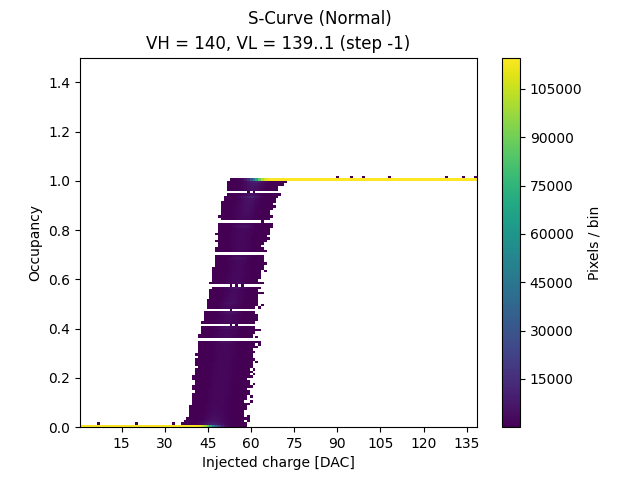
\includegraphics[scale=.6]{all_norm_thscan_140}
\caption{S-curves of all pixels of the Normal FE with an injection pulse of 140 DAC.}
\label{fig:norm_scurve_140}
\end{figure}

Using this setting, none of the pixels were noisy and so it wasn't necessary introduce (use, ...) any mask.

As already explained in the previous section (reference?) the threshold distributions from the two different measurements with an injection pulse of 140 and 200 DAC respectively, have been fitted and they are showed in figure \vref{fig:thdist_norm}

\begin{figure}[h!]
\centering
\subfigure[VH = 140 DAC]
{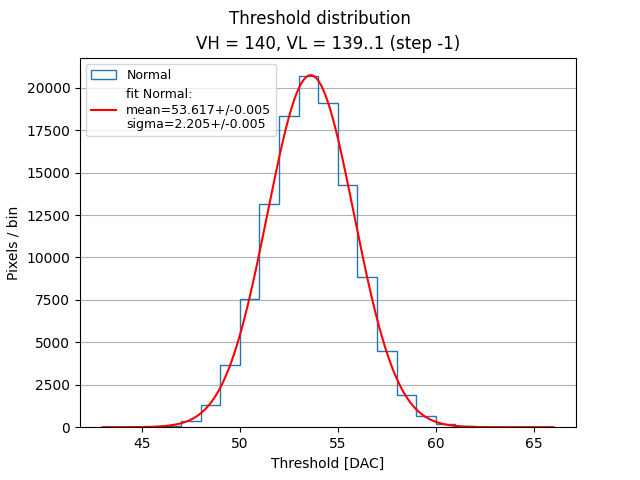
\includegraphics[scale=0.6]{all_norm_thdist_140}}\quad
\subfigure[VH = 200 DAC]
{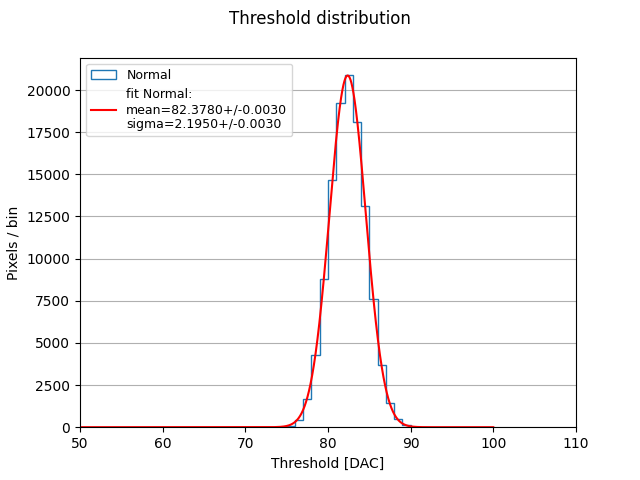
\includegraphics[scale=0.6]{all_norm_thdist_200}}\\
\caption{Threshold distributions of \textbf{Normal} flavor before and at the maximum saturation, respectively.}
\label{fig:thdist_norm}
\end{figure}
 
For the greater (higher) injection height, 8 different measurement have be actually done, each one on 28 consecutive columns and on all rows. Then data have been put together to obtain a single (summary) plot on the whole flavor. Same procedure has been preformed on the \textbf{Cascode FE}.


\subsubsection{Cascode FE}

\textbf{Cascode FE} is the second flavor and like \textbf{Normal FE} it consists of 512 rows (0-511) and 224 columns (224-447) for a number of total pixels equal to 114.688. Also for this study (measurement) the same values' registers of the setting used during the Test Beam in Desy (table \vref{tab:tb_settings}) have been used and there weren't find noisy pixels. 
In figure \vref{fig:casc_curve_140} the S-curves of all pixels ar showed.

\begin{figure}[h!]
\centering
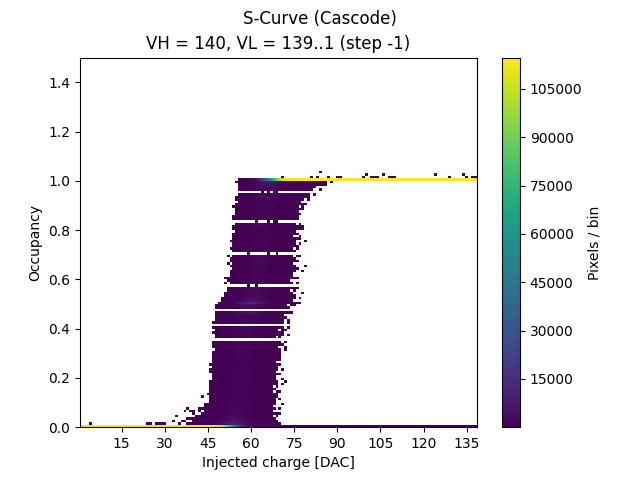
\includegraphics[scale=.6]{all_casc_thscan_140}
\caption{S-curves of all pixels in the \textbf{Cascode} flavor with an injection pulse of 140 DAC.}
\label{fig:casc_scurve_140}
\end{figure}

The fit of the threshold distributions instead, are showed in figure \vref{fig:thdist_casc}.

\begin{figure}[h!]
\centering
\subfigure[VH = 140 DAC]
{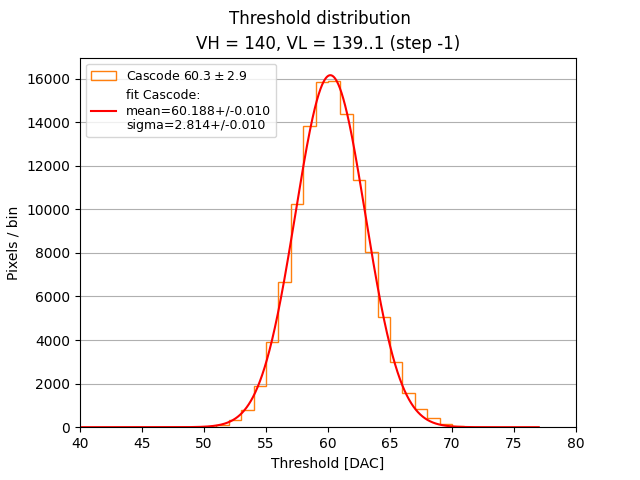
\includegraphics[scale=0.6]{all_casc_thdist_140}}\quad
\subfigure[VH = 200 DAC]
{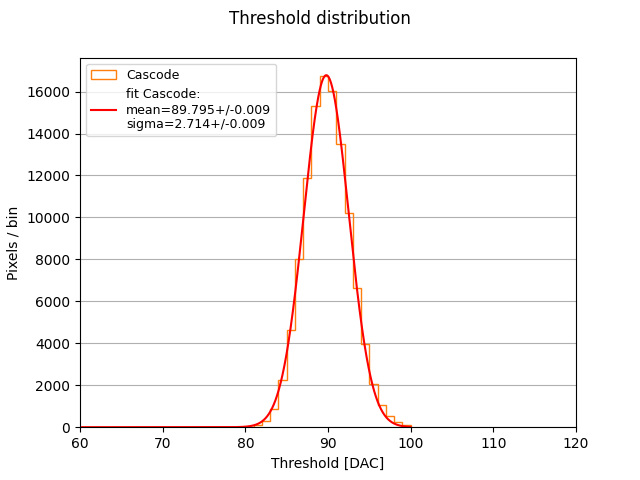
\includegraphics[scale=0.6]{all_casc_thdist_200}}\\
\caption{Threshold distributions of \textbf{Cascode} flavor before and at the maximum saturation, respectively.}
\label{fig:thdist_casc}
\end{figure}


\subsubsection{HV-Cascode FE}

The third flavor is \textbf{HV-Cascode FE} where HV stands for \textbf{High Voltage} and it is formed (consists) of 512 rows (0-511) and 32 columns (448-479) for a total number of pixel equal to 16384. Also for these last two flavors, the main chip registers are set with the same values tested and used during the Test Beam (@Desy). They are reported in table \vref{tab:tb_hv_settings}.

\begin{table}[h!]
\centering
\begin{tabular}{c|c}
Registri & Default Settings (''GOE'') \\
\hline
ITHR & 30 \\
\hline
IBIAS & 60 \\
\hline
VRESET & 100 \\
\hline
ICASN & 8 \\
\hline
VCASP & 40 \\
\hline
VCASC & 228 \\
\hline
IDB & 100 \\
\hline
ITUNE & 53 \\
\hline
VCLIP & 255 \\
\hline
ICOMP & 80 \\
\hline
IDEL & 88 \\
\hline
IRAM & 50 \\
\hline
\end{tabular}
\caption{Settings of the main registers used for the W14R12 chip, for the HV's flavors, during the Test Beam in Desy.}
\label{tab:tb_hv_settings}
\end{table}

As we can see from the plot of the alle S-curves in figure \vref{fig:hvc_scurve_140}, with these choices of values' registers, there were a lot of noisy pixels, but at this stage of measurements, they were not masked.

\begin{figure}[h!]
\centering
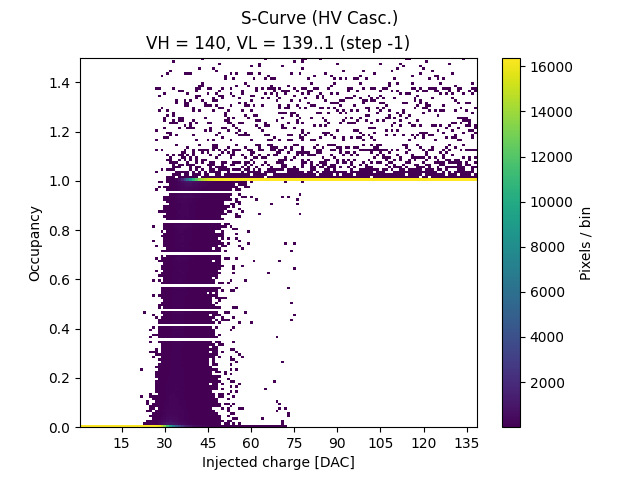
\includegraphics[scale=.6]{all_HVc_thscan_140}
\caption{S-curves of all pixels in \textbf{HV Cascode} flavor with an injection pulse of 140 DAC.}
\label{fig:hvc_scurve_140}
\end{figure}

In figure \vref{fig:thdist_hvc} are showed the fit of the threshold distributions for the two different injections pulse.

\begin{figure}[h!]
\centering
\subfigure[VH = 140 DAC]
{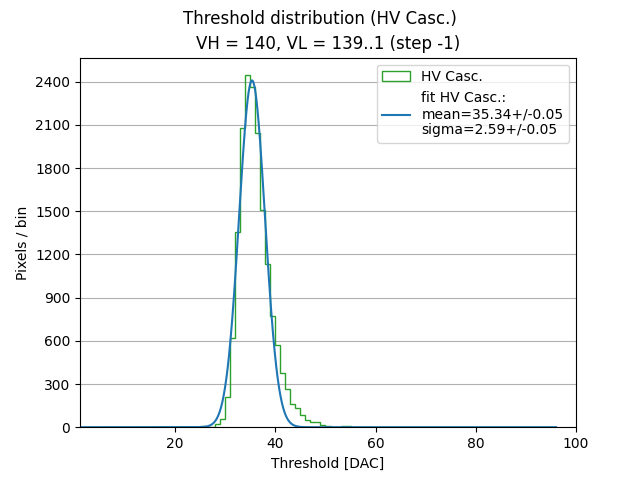
\includegraphics[scale=0.6]{all_HVc_thdist_140}}\quad
\subfigure[VH = 200 DAC]
{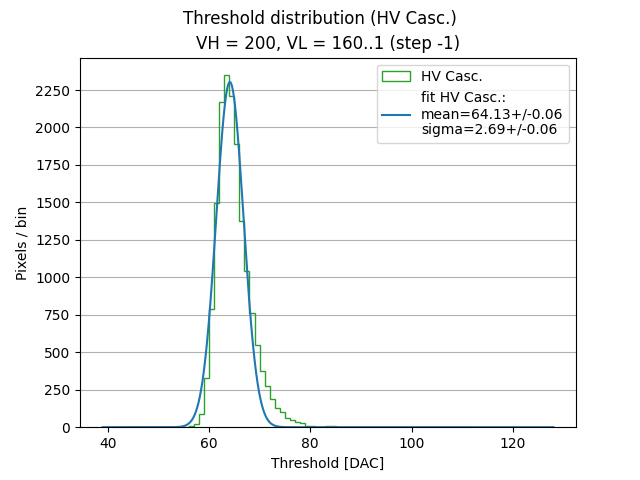
\includegraphics[scale=0.6]{all_HVc_thdist_200}}\\
\caption{Threshold distributions of \textbf{HV Cascode} flavor before and at the maximum saturation, respectively.}
\label{fig:thdist_hvc}
\end{figure}


\subsubsection{HV-Normal FE}

The fourth and last flavor is the \textbf{HV-Normal FE} which consists of 512 rows (0-511) and 32 columns (479-511) for a total number of pixel equal to 16.384. The main registers have been set with the values reported in table \vref{tab:tb_hv_settings}.
In figure \vref{fig:hv_scurve_140}, the S-curves of all pixel in the flavor. Also here we can see that there were some noisy pixels unmasked.
Moreover, in this final flavor, the last 16 columns were not working and as a matter of fact they had return a peak of threshold near the value 0, which is excluded from the threshold distributions plots.

So actually in this part of the matrix, the real number of pixel studied was the half of the total, such as 8192 pixels.



\begin{figure}[h!]
\centering
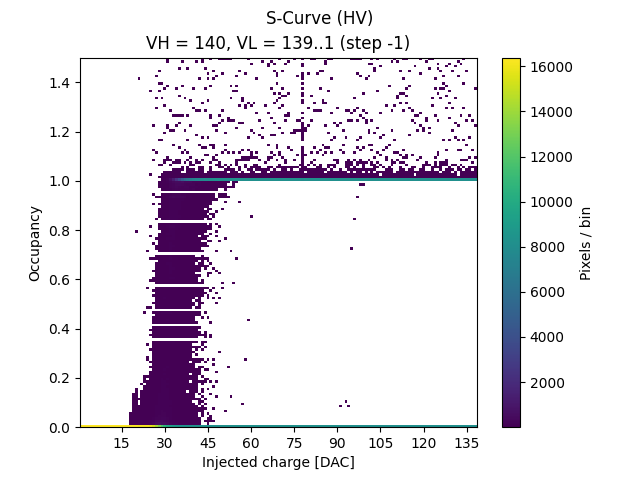
\includegraphics[scale=.6]{all_HV_thscan_140}
\caption{S-curves of all pixels in \textbf{HV Cascode FE} with an injection pulse of 140 DAC.}
\label{fig:hv_scurve_140}
\end{figure}

In figure \vref{fig:thdist_hvc} the fit of the threshold distributions for the two different values of injection height are reported.


\begin{figure}[h!]
\centering
\subfigure[VH = 140 DAC]
{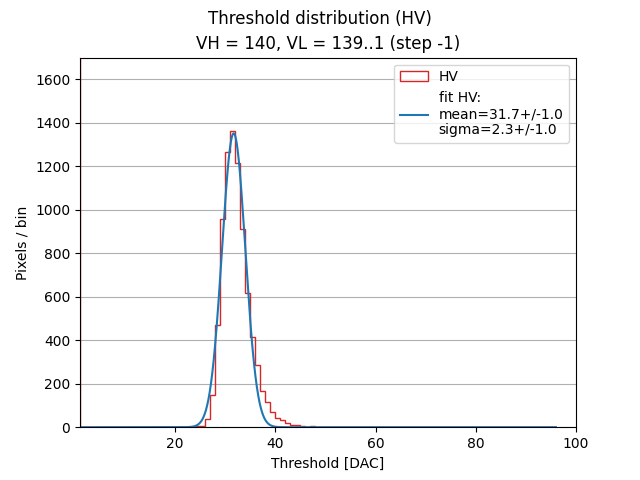
\includegraphics[scale=0.6]{all_HV_thdist_140}}\quad
\subfigure[VH = 200 DAC]
{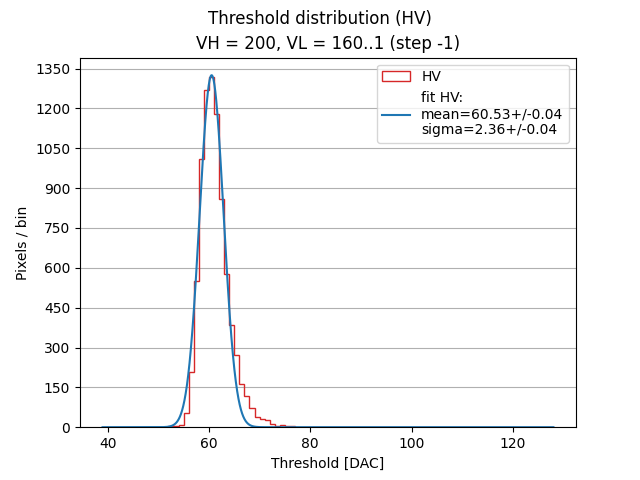
\includegraphics[scale=0.6]{all_HV_thdist_200}}\\
\caption{Threshold distributions of \textbf{HV} flavor before and at the maximum saturation, respectively.}
\label{fig:thdist_hvc}
\end{figure}



\subsection{Noise and Equivalent Noise Charge (ENC)}
%\addcontentsline{toc}{subsection}{Noise and Equivalent Noise Charge (ENC)}

\subsection{Curve del Time Over Threshold (TOT) e fit}
%\addcontentsline{toc}{subsection}{Curve del Time Over Threshold (TOT) e fit}

\section{Caratterizzazione con le sorgenti radioattive}
%\addcontentsline{toc}{section}{Caratterizzazione con le sorgenti radioattive}

Fe55, Am241, Cd109, Sr190

\subsection{Calibrazione della capacità di iniezione}
%\addcontentsline{toc}{subsection}{Calibrazione della capacità di iniezione}
